\documentclass[11pt,a4paperpaper,]{report}
\usepackage{lmodern}
\usepackage{amssymb,amsmath}
\usepackage{ifxetex,ifluatex}
\usepackage{fixltx2e} % provides \textsubscript
\ifnum 0\ifxetex 1\fi\ifluatex 1\fi=0 % if pdftex
  \usepackage[T1]{fontenc}
  \usepackage[utf8]{inputenc}
\else % if luatex or xelatex
  \ifxetex
    \usepackage{mathspec}
  \else
    \usepackage{fontspec}
  \fi
  \defaultfontfeatures{Ligatures=TeX,Scale=MatchLowercase}
\fi
% use upquote if available, for straight quotes in verbatim environments
\IfFileExists{upquote.sty}{\usepackage{upquote}}{}
% use microtype if available
\IfFileExists{microtype.sty}{%
\usepackage{microtype}
\UseMicrotypeSet[protrusion]{basicmath} % disable protrusion for tt fonts
}{}
\usepackage{hyperref}
\hypersetup{unicode=true,
            pdfborder={0 0 0},
            breaklinks=true}
\urlstyle{same}  % don't use monospace font for urls
\usepackage{longtable,booktabs}
\IfFileExists{parskip.sty}{%
\usepackage{parskip}
}{% else
\setlength{\parindent}{0pt}
\setlength{\parskip}{6pt plus 2pt minus 1pt}
}
\setlength{\emergencystretch}{3em}  % prevent overfull lines
\providecommand{\tightlist}{%
  \setlength{\itemsep}{0pt}\setlength{\parskip}{0pt}}
\setcounter{secnumdepth}{5}
% Redefines (sub)paragraphs to behave more like sections
\ifx\paragraph\undefined\else
\let\oldparagraph\paragraph
\renewcommand{\paragraph}[1]{\oldparagraph{#1}\mbox{}}
\fi
\ifx\subparagraph\undefined\else
\let\oldsubparagraph\subparagraph
\renewcommand{\subparagraph}[1]{\oldsubparagraph{#1}\mbox{}}
\fi


% Table of contents formatting
\renewcommand{\contentsname}{Table of Contents}
\setcounter{tocdepth}{3}

% Headers and page numbering
\usepackage{fancyhdr}
\usepackage{tgadventor}

\pagestyle{plain}

% Following package is used to add background image to front page
\usepackage{wallpaper}

% Table package
\usepackage{ctable}% http://ctan.org/pkg/ctable

% Deal with 'LaTeX Error: Too many unprocessed floats.'
\usepackage{morefloats}
% or use \extrafloats{100}
% add some \clearpage

% % Chapter header
% \usepackage{titlesec, blindtext, color}
% \definecolor{gray75}{gray}{0.75}
% \newcommand{\hsp}{\hspace{20pt}}
% \titleformat{\chapter}[hang]{\Huge\bfseries}{\thechapter\hsp\textcolor{gray75}{|}\hsp}{0pt}{\Huge\bfseries}

% % Fonts and typesetting
% \setmainfont[Scale=1.1]{Helvetica}
% \setsansfont[Scale=1.1]{Verdana}

% FONTS
\usepackage{xunicode}
\usepackage{xltxtra}
\fontfamily{Fourier}
\defaultfontfeatures{Mapping=tex-text} % converts LaTeX specials (``quotes'' --- dashes etc.) to unicode
% \setromanfont[Scale=1.01,Ligatures={Common},Numbers={OldStyle}]{Palatino}
% \setromanfont[Scale=1.01,Ligatures={Common},Numbers={OldStyle}]{Adobe Caslon Pro}
%Following line controls size of code chunks
% \setmonofont[Scale=0.9]{Monaco}
%Following line controls size of figure legends
% \setsansfont[Scale=1.2]{Optima Regular}
% \usepackage{tgadventor}
% \usepackage[T1]{fontenc}

%Attempt to set math size
%First size must match the text size in the document or command will not work
%\DeclareMathSizes{display size}{text size}{script size}{scriptscript size}.
\DeclareMathSizes{12}{13}{7}{7}

% ---- CUSTOM AMPERSAND
% \newcommand{\amper}{{\fontspec[Scale=.95]{Adobe Caslon Pro}\selectfont\itshape\&}}

% HEADINGS
\usepackage{sectsty}
\usepackage[normalem]{ulem}
\sectionfont{\rmfamily\mdseries\Large}
\subsectionfont{\rmfamily\mdseries\scshape\large}
\subsubsectionfont{\rmfamily\bfseries\upshape\large}
% \sectionfont{\rmfamily\mdseries\Large}
% \subsectionfont{\rmfamily\mdseries\scshape\normalsize}
% \subsubsectionfont{\rmfamily\bfseries\upshape\normalsize}

% Set figure legends and captions to be smaller sized sans serif font
\usepackage[font={footnotesize,sf}]{caption}

\usepackage{siunitx}

% Adjust spacing between lines to 1.5
\usepackage{setspace}
\onehalfspacing
% \doublespacing
\raggedbottom

% Set margins
\usepackage[top=1.2in,bottom=1.2in,left=1.1in,right=1.0in]{geometry}
% \setlength\parindent{0.4in} % indent at start of paragraphs (set to 0.3?)
\setlength{\parskip}{9pt}

% Add space between pararaphs
% http://texblog.org/2012/11/07/correctly-typesetting-paragraphs-in-latex/
% \usepackage{parskip}
% \setlength{\parskip}{\baselineskip}

% Set colour of links to black so that they don't show up when printed
\usepackage{hyperref}
\hypersetup{colorlinks=false, linkcolor=black}

% Tables
\usepackage{booktabs}
\usepackage{threeparttable}
\usepackage{array}
\newcolumntype{x}[1]{%
>{\centering\arraybackslash}m{#1}}%

% Allow for long captions and float captions on opposite page of figures
% \usepackage[rightFloats, CaptionBefore]{fltpage}

% Don't let floats cross subsections
% \usepackage[section,subsection]{extraplaceins}

\date{}

\begin{document}

\begin{titlepage}
    \begin{center}


        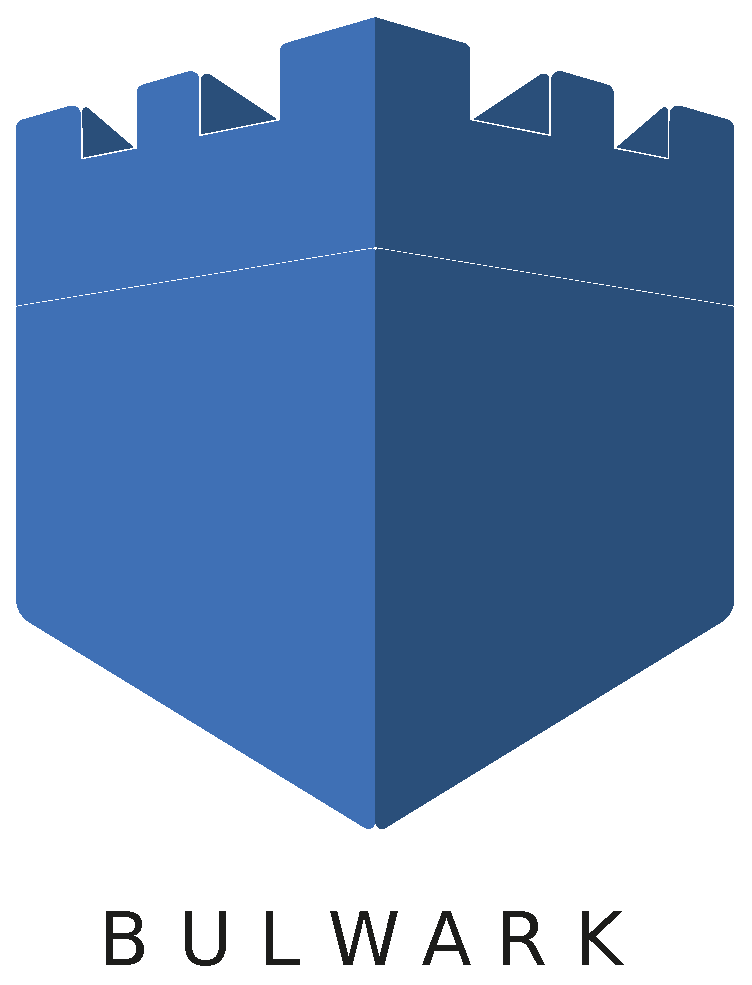
\includegraphics[width=0.4\textwidth]{style/bulwark.eps}

        \vspace*{2.5cm}

        \huge
        Bulwark Cryptocurrency Whitepaper

        \vspace{1.5cm}

        \vfill

        \normalsize
        Bulwark Core Team:\\
        Levi (Project Director)\\
        Jack (Marketing Director)\\
        Stu (Blockchain Developer)\\
        Dustin (Full-Stack Developer)\\
        Kewagi (Software Engineer)\\
        Patrick (Brand and Design Manager)\\
        Voxterra (Community Manager)\\
        \vspace{0.8cm}

        % Uncomment the following line
        % to add a centered university logo


        \normalsize
        The Bulwark Core Team\\
        October 2018

    \normalsize
    Version 1.4
        % Except where otherwise noted, content in this thesis is licensed under a Creative Commons Attribution 4.0 License (http://creativecommons.org/licenses/by/4.0), which permits unrestricted use, distribution, and reproduction in any medium, provided the original work is properly cited.

    \end{center}
\end{titlepage}

\vspace*{\fill}

\noindent
\textit{
We, The Bulwark Core Team, confirm that the work presented in this whitepaper is our own. Where information has been derived from other sources, we confirm that this has been indicated in the attributions.
} \vspace*{\fill} \pagenumbering{gobble}

\chapter*{Abstract}\label{abstract}
\addcontentsline{toc}{chapter}{Abstract}

Bulwark (ticker: BWK) is a community-oriented coin born out of an
observation of generally unfair practices within the masternode privacy
coin space. Our deliberate, fair, launch strategy allows participants
the opportunity to join a promising project at inception. We offer a
simple value proposition with no grandiose promise: we will deliver a
privacy coin that works today and into the future by leveraging
best-practices from both DASH and PIVX. No fanciful visions with a
limited prospect of delivery, but a working coin on a working platform
with support into the future. This does not mean we plan no innovation,
but instead that we will deliver results rather than hype. Bulwark's
main focus will be on a number of privacy hardware developments that
will expand upon the capabilities of our blockchain while also offering
additional privacy enhancements for those that choose to build or
acquire them. With no ICO, a soft-launch reward ramp, small premine, and
miner-favored block reward allocations, Bulwark adopters will have
ground-floor access to a privacy coin offering a blend of masternodes
and the best available privacy hardware technology alongside a
meaningful development roadmap. Masternodes will be available, and
functioning, on launch and are a fundamental part of this coin's vision
and will stabilize circulation, secure the network, and provide
important functionality. \pagenumbering{roman} \setcounter{page}{1}

\chapter*{Acknowledgements}\label{acknowledgements}
\addcontentsline{toc}{chapter}{Acknowledgements}

Bulwark would not have been possible without the prior works of the
respective Bitcoin, Peercoin, Blackcoin, Talkcoin, Dash and PIVX teams.
Open source software and its contributors are constantly paving the way
toward new and exciting innovations. When information and knowledge are
free to build upon, society as a whole benefits. We are grateful to our
predecessors for the opportunity to contribute to this growing
ecosystem.

\newpage

\pagenumbering{gobble}

\tableofcontents

\newpage

\chapter*{Abbreviations}\label{abbreviations}
\addcontentsline{toc}{chapter}{Abbreviations}

\begin{tabbing}
\textbf{ASIC}~~~~~~~~~~~    \= \textbf{A}pplication-\textbf{S}pecific \textbf{I}ntegrated \textbf{C}ircuit\\
\textbf{CPU}    \> \textbf{C}entral \textbf{P}rocessing \textbf{U}nit \\
\textbf{CAD}    \> \textbf{C}omputer \textbf{A}ided \textbf{D}esign \\
\textbf{BWK}    \> \textbf{B}ul\textbf{w}ar\textbf{k} Cryptocurrency \\
\textbf{TOR}    \> \textbf{T}he \textbf{O}nion \textbf{R}outer \\
\textbf{MN} \> \textbf{M}aster\textbf{N}ode \\
\textbf{BR} \> \textbf{B}lock \textbf{R}eward \\
\textbf{UI} \> \textbf{U}ser \textbf{I}nterface \\
\textbf{UX} \> \textbf{U}ser E\textbf{x}perience \\
\end{tabbing}

\newpage

\setcounter{page}{1} \renewcommand{\thepage}{\arabic{page}}

\chapter{Brief Introduction to
Cryptocurrency}\label{brief-introduction-to-cryptocurrency}

\section{Background}\label{background}

In 2009, Satoshi Nakamoto released a paper entitled
\textit{Bitcoin: A Peer-to-Peer Electronic Cash System} detailing his
vision of commerce. Nakamoto's vision detailed a peer-to-peer currency
system backed by a hash based proof-of-work. The network would timestamp
transactions by hashing them into an ongoing ledger that could not be
changed without redoing the proof-of-work. Nodes would choose the
longest chain as proof of events witnessed by the largest pool of
hashing power. As long as \(\geq\) 51\% of the network hashing power is
controlled by nodes not intending to facilitate an attack, the chain
they generate will remain the longest. (Nakamoto 2009)

\section{The Block}\label{the-block}

Each block on the network is prefaced with an 80 byte header containing
a double SHA256 hashed copy of the previous block's header, merkle root
(a double SHA256 hashed derivation of all the hashes that occurred in
the block), the time stamp at which proof-of-work began, difficulty
target this header's hash must be less-than or equal to, and the nonce
at which miners reached the difficulty target. As such, any attempts to
modify any transaction in any block will result in the rejection of the
block by the network's miners. (Bitcoin Core Team 2017)

\section{The Blockchain}\label{the-blockchain}

Groups of transactions are formed into blocks and those blocks are
placed chronologically into a chain - forming the blockchain. The
blockchain creates a moving history of all of the activity within the
network and serves as a distributed consensus model where any
transaction can be verified at any time (Crosby et al. 2015).

\section{Proof-Of-Work}\label{proof-of-work}

Proof-of-Work is a system of verification in which miners must devote
tangible resources (electricity, hardware costs) to solve an arbitrary
probabilistic \textit{word puzzle}. In order for a bad actor to taint
the blockchain with a fraudulent transaction, they must complete all
proof-of-work up to the present point. (Okupski 2016)

Note: Bulwark is no longer Proof Of Work and transitioned into Proof of
Stake in June 2018.

\section{Proof-Of-Stake}\label{proof-of-stake}

Proof-of-Stake is a competition between shareholders, where based on
connectivity to the network and random chance, you can receive new coins
to assist in the decentralization of the network. Proof-Of-Stake is far
more energy efficient in that it requires no dedicated hardware and
negligible amounts of electricity to reward miners, and in many cases is
far more resilient to a 51\% attack on the network. (Blackcoin Core Team
2016)

\chapter{Introducing Bulwark}\label{introducing-bulwark}

\section{A solid foundation}\label{a-solid-foundation}

Every home needs a solid foundation, and Bulwark is no different.
Bulwark is built upon \textit{PIVX}, which itself is built upon the
popular \textit{DASH} cryptocurrency. While lineages can all be traced
back to the original Satoshi Core, each project has chosen a particular
direction with goals and ideals that represent the communities they
serve. We will extend, and place emphasis on, the privacy coin features
of our predecessor platforms by exploring new technologies, while
creating tool sets and opportunities for Bulwark's integration into
present day technology platforms.

\section{A team dedicated to the
community}\label{a-team-dedicated-to-the-community}

For some projects, communities are an afterthought. Bulwark's number one
priority is the community. With giveaways, contests, a lively discussion
platform and a zero-tolerance policy toward the harassment of newcomers,
Bulwark strives to be the cryptocurrency for all varieties of end-users.
Members of our userbase are already contributing useful scripts and
guides to further enhance the user experience.

\section{Fair and balanced}\label{fair-and-balanced}

At the time of writing, there have been an influx of cryptocurrencies
utilizing a similar foundation. While the underlying technology is
solid, oftentimes a deeper examination of their specifications and
blockchain parameters reveals less-than-fair practices.

\section{Fast and functional}\label{fast-and-functional}

With a 90 second block time, masternode consensus and transaction
locking, reasonable emissions schedule, and eco-friendly staking,
Bulwark aspires to be a truly fast and functional cryptocurrency.

\section{Privacy Hardware
Development}\label{privacy-hardware-development}

Bulwark has elected to put its primary focus on developing a number of
privacy hardware developments to enhance a user's abilities to retain
their freedom and privacy while providing a justifiable price point.
Some of these developments are discussed more in depth in Chapter 7 (The
Future) and include staking boxes, secure local masternode hosting
solutions, hardware wallets, and network routers.

\chapter{Our Blockchain Parameters.}\label{our-blockchain-parameters.}

\section{Bulwark Specifications at a
Glance}\label{bulwark-specifications-at-a-glance}

\ref{ref_a_table}

\begin{longtable}[c]{@{}ll@{}}
\caption{At a glance specifications for Bulwark
\label{ref_a_table}}\tabularnewline
\toprule
\begin{minipage}[b]{0.35\columnwidth}\raggedright\strut
Specification
\strut\end{minipage} &
\begin{minipage}[b]{0.59\columnwidth}\raggedright\strut
Descriptor
\strut\end{minipage}\tabularnewline
\midrule
\endfirsthead
\toprule
\begin{minipage}[b]{0.35\columnwidth}\raggedright\strut
Specification
\strut\end{minipage} &
\begin{minipage}[b]{0.59\columnwidth}\raggedright\strut
Descriptor
\strut\end{minipage}\tabularnewline
\midrule
\endhead
\begin{minipage}[t]{0.35\columnwidth}\raggedright\strut
Ticker
\strut\end{minipage} &
\begin{minipage}[t]{0.59\columnwidth}\raggedright\strut
BWK
\strut\end{minipage}\tabularnewline
\begin{minipage}[t]{0.35\columnwidth}\raggedright\strut
Algorithm
\strut\end{minipage} &
\begin{minipage}[t]{0.59\columnwidth}\raggedright\strut
NIST5
\strut\end{minipage}\tabularnewline
\begin{minipage}[t]{0.35\columnwidth}\raggedright\strut
RPC Port
\strut\end{minipage} &
\begin{minipage}[t]{0.59\columnwidth}\raggedright\strut
52541
\strut\end{minipage}\tabularnewline
\begin{minipage}[t]{0.35\columnwidth}\raggedright\strut
P2P Port
\strut\end{minipage} &
\begin{minipage}[t]{0.59\columnwidth}\raggedright\strut
52543
\strut\end{minipage}\tabularnewline
\begin{minipage}[t]{0.35\columnwidth}\raggedright\strut
Block Spacing
\strut\end{minipage} &
\begin{minipage}[t]{0.59\columnwidth}\raggedright\strut
90 Seconds
\strut\end{minipage}\tabularnewline
\begin{minipage}[t]{0.35\columnwidth}\raggedright\strut
Difficulty Algorithm
\strut\end{minipage} &
\begin{minipage}[t]{0.59\columnwidth}\raggedright\strut
Dark Gravity Wave v3.0
\strut\end{minipage}\tabularnewline
\begin{minipage}[t]{0.35\columnwidth}\raggedright\strut
Block Size
\strut\end{minipage} &
\begin{minipage}[t]{0.59\columnwidth}\raggedright\strut
1MB
\strut\end{minipage}\tabularnewline
\begin{minipage}[t]{0.35\columnwidth}\raggedright\strut
Mined/Minted Maturity
\strut\end{minipage} &
\begin{minipage}[t]{0.59\columnwidth}\raggedright\strut
67 Blocks (\textasciitilde{}100 Minutes)
\strut\end{minipage}\tabularnewline
\begin{minipage}[t]{0.35\columnwidth}\raggedright\strut
Confirmation
\strut\end{minipage} &
\begin{minipage}[t]{0.59\columnwidth}\raggedright\strut
6 Blocks (\textasciitilde{}9 Minutes)
\strut\end{minipage}\tabularnewline
\begin{minipage}[t]{0.35\columnwidth}\raggedright\strut
Circulation (1 Year)
\strut\end{minipage} &
\begin{minipage}[t]{0.59\columnwidth}\raggedright\strut
14,505,720 BWK
\strut\end{minipage}\tabularnewline
\begin{minipage}[t]{0.35\columnwidth}\raggedright\strut
Circulation (5 Years)
\strut\end{minipage} &
\begin{minipage}[t]{0.59\columnwidth}\raggedright\strut
27,668,220 BWK
\strut\end{minipage}\tabularnewline
\begin{minipage}[t]{0.35\columnwidth}\raggedright\strut
PoW Period
\strut\end{minipage} &
\begin{minipage}[t]{0.59\columnwidth}\raggedright\strut
\textit{nHeight} \(\leq\) 182,700
\strut\end{minipage}\tabularnewline
\begin{minipage}[t]{0.35\columnwidth}\raggedright\strut
PoS Period
\strut\end{minipage} &
\begin{minipage}[t]{0.59\columnwidth}\raggedright\strut
\textit{nHeight} \(\geq\) 182,701
\strut\end{minipage}\tabularnewline
\begin{minipage}[t]{0.35\columnwidth}\raggedright\strut
Protocol Support
\strut\end{minipage} &
\begin{minipage}[t]{0.59\columnwidth}\raggedright\strut
IPV4, IPV6, TOR
\strut\end{minipage}\tabularnewline
\begin{minipage}[t]{0.35\columnwidth}\raggedright\strut
PoS
\strut\end{minipage} &
\begin{minipage}[t]{0.59\columnwidth}\raggedright\strut
Blackcoin v3.0 PoS
\strut\end{minipage}\tabularnewline
\bottomrule
\end{longtable}

\newpage

\section{SlowStart}\label{slowstart}

Our fair start is provided with the following code snippet (Credit:
ZCash).

\begin{verbatim}

        int64_t nSlowSubsidy = 50 * COIN;

        if (nHeight < 960 / 2) {        // If block height less than 480,
           nSlowSubsidy /= 960;         // Set nSubsidy to .05208333
           nSlowSubsidy *= nHeight;     // Multiply present height by .05208333
        } else if (nHeight < 960 {      // ex: Block 200, BR will be 10.41666600
            nSlowSubsidy /= 960;        // Credits: ZCASH Team
            nSlowSubsidy *= nHeight;
\end{verbatim}

The slow start period averages at 25 coins per block at block 960.

\section{Dark Gravity Wave 3.0}\label{dark-gravity-wave-3.0}

Dark Gravity Wave is employed by Bulwark from the start as a method of
retargeting PoW difficulty. It uses a simple moving average that can
respond to large nethash increases or drop-offs in just a few blocks.
This alleviates the ``stuck block effect'' often caused by multipools
and prevents one person adding a substantial amount of computing power
from instantly solving more than a few blocks.

\chapter{Block Rewards}\label{block-rewards}

\section{PoW Block Rewards}\label{pow-block-rewards}

\begin{longtable}[c]{@{}lllcl@{}}
\toprule
\begin{minipage}[b]{0.16\columnwidth}\raggedright\strut
Subsidy
\strut\end{minipage} &
\begin{minipage}[b]{0.19\columnwidth}\raggedright\strut
Block
\strut\end{minipage} &
\begin{minipage}[b]{0.10\columnwidth}\raggedright\strut
PoW
\strut\end{minipage} &
\begin{minipage}[b]{0.10\columnwidth}\centering\strut
MN
\strut\end{minipage} &
\begin{minipage}[b]{0.16\columnwidth}\raggedright\strut
Circulation
\strut\end{minipage}\tabularnewline
\midrule
\endhead
\begin{minipage}[t]{0.16\columnwidth}\raggedright\strut
489720
\strut\end{minipage} &
\begin{minipage}[t]{0.19\columnwidth}\raggedright\strut
1
\strut\end{minipage} &
\begin{minipage}[t]{0.10\columnwidth}\raggedright\strut
100\%
\strut\end{minipage} &
\begin{minipage}[t]{0.10\columnwidth}\centering\strut
NA
\strut\end{minipage} &
\begin{minipage}[t]{0.16\columnwidth}\raggedright\strut
489200
\strut\end{minipage}\tabularnewline
\begin{minipage}[t]{0.16\columnwidth}\raggedright\strut
\textasciitilde{}25(avg)
\strut\end{minipage} &
\begin{minipage}[t]{0.19\columnwidth}\raggedright\strut
2-960
\strut\end{minipage} &
\begin{minipage}[t]{0.10\columnwidth}\raggedright\strut
100\%
\strut\end{minipage} &
\begin{minipage}[t]{0.10\columnwidth}\centering\strut
NA
\strut\end{minipage} &
\begin{minipage}[t]{0.16\columnwidth}\raggedright\strut
513150
\strut\end{minipage}\tabularnewline
\begin{minipage}[t]{0.16\columnwidth}\raggedright\strut
50.000
\strut\end{minipage} &
\begin{minipage}[t]{0.19\columnwidth}\raggedright\strut
961-28800
\strut\end{minipage} &
\begin{minipage}[t]{0.10\columnwidth}\raggedright\strut
80\%
\strut\end{minipage} &
\begin{minipage}[t]{0.10\columnwidth}\centering\strut
20\%
\strut\end{minipage} &
\begin{minipage}[t]{0.16\columnwidth}\raggedright\strut
1953150
\strut\end{minipage}\tabularnewline
\begin{minipage}[t]{0.16\columnwidth}\raggedright\strut
50.000
\strut\end{minipage} &
\begin{minipage}[t]{0.19\columnwidth}\raggedright\strut
28801-57600
\strut\end{minipage} &
\begin{minipage}[t]{0.10\columnwidth}\raggedright\strut
75\%
\strut\end{minipage} &
\begin{minipage}[t]{0.10\columnwidth}\centering\strut
25\%
\strut\end{minipage} &
\begin{minipage}[t]{0.16\columnwidth}\raggedright\strut
3393150
\strut\end{minipage}\tabularnewline
\begin{minipage}[t]{0.16\columnwidth}\raggedright\strut
50.000
\strut\end{minipage} &
\begin{minipage}[t]{0.19\columnwidth}\raggedright\strut
57601-86400
\strut\end{minipage} &
\begin{minipage}[t]{0.10\columnwidth}\raggedright\strut
66\%
\strut\end{minipage} &
\begin{minipage}[t]{0.10\columnwidth}\centering\strut
33\%
\strut\end{minipage} &
\begin{minipage}[t]{0.16\columnwidth}\raggedright\strut
4833150
\strut\end{minipage}\tabularnewline
\begin{minipage}[t]{0.16\columnwidth}\raggedright\strut
43.750
\strut\end{minipage} &
\begin{minipage}[t]{0.19\columnwidth}\raggedright\strut
86401-172800
\strut\end{minipage} &
\begin{minipage}[t]{0.10\columnwidth}\raggedright\strut
50\%
\strut\end{minipage} &
\begin{minipage}[t]{0.10\columnwidth}\centering\strut
50\%
\strut\end{minipage} &
\begin{minipage}[t]{0.16\columnwidth}\raggedright\strut
8613150
\strut\end{minipage}\tabularnewline
\begin{minipage}[t]{0.16\columnwidth}\raggedright\strut
37.500
\strut\end{minipage} &
\begin{minipage}[t]{0.19\columnwidth}\raggedright\strut
172801-182700
\strut\end{minipage} &
\begin{minipage}[t]{0.10\columnwidth}\raggedright\strut
50\%
\strut\end{minipage} &
\begin{minipage}[t]{0.10\columnwidth}\centering\strut
50\%
\strut\end{minipage} &
\begin{minipage}[t]{0.16\columnwidth}\raggedright\strut
371212
\strut\end{minipage}\tabularnewline
\bottomrule
\end{longtable}

\newpage

\section{PoS Block Rewards}\label{pos-block-rewards}

\begin{longtable}[c]{@{}llll@{}}
\caption{PoS Period Block Reward Specifications
\label{ref_c_table}}\tabularnewline
\toprule
\begin{minipage}[b]{0.12\columnwidth}\raggedright\strut
Subsidy
\strut\end{minipage} &
\begin{minipage}[b]{0.22\columnwidth}\raggedright\strut
Block
\strut\end{minipage} &
\begin{minipage}[b]{0.15\columnwidth}\raggedright\strut
Budget
\strut\end{minipage} &
\begin{minipage}[b]{0.27\columnwidth}\raggedright\strut
MN / PoS
\strut\end{minipage}\tabularnewline
\midrule
\endfirsthead
\toprule
\begin{minipage}[b]{0.12\columnwidth}\raggedright\strut
Subsidy
\strut\end{minipage} &
\begin{minipage}[b]{0.22\columnwidth}\raggedright\strut
Block
\strut\end{minipage} &
\begin{minipage}[b]{0.15\columnwidth}\raggedright\strut
Budget
\strut\end{minipage} &
\begin{minipage}[b]{0.27\columnwidth}\raggedright\strut
MN / PoS
\strut\end{minipage}\tabularnewline
\midrule
\endhead
\begin{minipage}[t]{0.12\columnwidth}\raggedright\strut
37.500
\strut\end{minipage} &
\begin{minipage}[t]{0.22\columnwidth}\raggedright\strut
182701-199999
\strut\end{minipage} &
\begin{minipage}[t]{0.15\columnwidth}\raggedright\strut
0\%
\strut\end{minipage} &
\begin{minipage}[t]{0.27\columnwidth}\raggedright\strut
\textit{SeeSaw}
\strut\end{minipage}\tabularnewline
\begin{minipage}[t]{0.12\columnwidth}\raggedright\strut
37.500
\strut\end{minipage} &
\begin{minipage}[t]{0.22\columnwidth}\raggedright\strut
200000-259200
\strut\end{minipage} &
\begin{minipage}[t]{0.15\columnwidth}\raggedright\strut
0\%
\strut\end{minipage} &
\begin{minipage}[t]{0.27\columnwidth}\raggedright\strut
65\% MN / 35\% PoS
\strut\end{minipage}\tabularnewline
\begin{minipage}[t]{0.12\columnwidth}\raggedright\strut
31.250
\strut\end{minipage} &
\begin{minipage}[t]{0.22\columnwidth}\raggedright\strut
259201-345600
\strut\end{minipage} &
\begin{minipage}[t]{0.15\columnwidth}\raggedright\strut
0\%
\strut\end{minipage} &
\begin{minipage}[t]{0.27\columnwidth}\raggedright\strut
65\% MN / 35\% PoS
\strut\end{minipage}\tabularnewline
\begin{minipage}[t]{0.12\columnwidth}\raggedright\strut
25.000
\strut\end{minipage} &
\begin{minipage}[t]{0.22\columnwidth}\raggedright\strut
345601-432000
\strut\end{minipage} &
\begin{minipage}[t]{0.15\columnwidth}\raggedright\strut
10\%
\strut\end{minipage} &
\begin{minipage}[t]{0.27\columnwidth}\raggedright\strut
60\% MN / 30\% PoS
\strut\end{minipage}\tabularnewline
\begin{minipage}[t]{0.12\columnwidth}\raggedright\strut
21.875
\strut\end{minipage} &
\begin{minipage}[t]{0.22\columnwidth}\raggedright\strut
432001-518400
\strut\end{minipage} &
\begin{minipage}[t]{0.15\columnwidth}\raggedright\strut
10\%
\strut\end{minipage} &
\begin{minipage}[t]{0.27\columnwidth}\raggedright\strut
60\% MN / 30\% PoS
\strut\end{minipage}\tabularnewline
\begin{minipage}[t]{0.12\columnwidth}\raggedright\strut
18.750
\strut\end{minipage} &
\begin{minipage}[t]{0.22\columnwidth}\raggedright\strut
518401-604800
\strut\end{minipage} &
\begin{minipage}[t]{0.15\columnwidth}\raggedright\strut
10\%
\strut\end{minipage} &
\begin{minipage}[t]{0.27\columnwidth}\raggedright\strut
60\% MN / 30\% PoS
\strut\end{minipage}\tabularnewline
\begin{minipage}[t]{0.12\columnwidth}\raggedright\strut
15.625
\strut\end{minipage} &
\begin{minipage}[t]{0.22\columnwidth}\raggedright\strut
604801-691200
\strut\end{minipage} &
\begin{minipage}[t]{0.15\columnwidth}\raggedright\strut
10\%
\strut\end{minipage} &
\begin{minipage}[t]{0.27\columnwidth}\raggedright\strut
60\% MN / 30\% PoS
\strut\end{minipage}\tabularnewline
\begin{minipage}[t]{0.12\columnwidth}\raggedright\strut
12.500
\strut\end{minipage} &
\begin{minipage}[t]{0.22\columnwidth}\raggedright\strut
691201-777600
\strut\end{minipage} &
\begin{minipage}[t]{0.15\columnwidth}\raggedright\strut
10\%
\strut\end{minipage} &
\begin{minipage}[t]{0.27\columnwidth}\raggedright\strut
60\% MN / 30\% PoS
\strut\end{minipage}\tabularnewline
\begin{minipage}[t]{0.12\columnwidth}\raggedright\strut
10.938
\strut\end{minipage} &
\begin{minipage}[t]{0.22\columnwidth}\raggedright\strut
777601-864000
\strut\end{minipage} &
\begin{minipage}[t]{0.15\columnwidth}\raggedright\strut
10\%
\strut\end{minipage} &
\begin{minipage}[t]{0.27\columnwidth}\raggedright\strut
60\% MN / 30\% PoS
\strut\end{minipage}\tabularnewline
\begin{minipage}[t]{0.12\columnwidth}\raggedright\strut
9.3750
\strut\end{minipage} &
\begin{minipage}[t]{0.22\columnwidth}\raggedright\strut
864001-950400
\strut\end{minipage} &
\begin{minipage}[t]{0.15\columnwidth}\raggedright\strut
10\%
\strut\end{minipage} &
\begin{minipage}[t]{0.27\columnwidth}\raggedright\strut
60\% MN / 30\% PoS
\strut\end{minipage}\tabularnewline
\begin{minipage}[t]{0.12\columnwidth}\raggedright\strut
7.8120
\strut\end{minipage} &
\begin{minipage}[t]{0.22\columnwidth}\raggedright\strut
950401-1036800
\strut\end{minipage} &
\begin{minipage}[t]{0.15\columnwidth}\raggedright\strut
10\%
\strut\end{minipage} &
\begin{minipage}[t]{0.27\columnwidth}\raggedright\strut
60\% MN / 30\% PoS
\strut\end{minipage}\tabularnewline
\begin{minipage}[t]{0.12\columnwidth}\raggedright\strut
6.2500
\strut\end{minipage} &
\begin{minipage}[t]{0.22\columnwidth}\raggedright\strut
1036801-1123200
\strut\end{minipage} &
\begin{minipage}[t]{0.15\columnwidth}\raggedright\strut
10\%
\strut\end{minipage} &
\begin{minipage}[t]{0.27\columnwidth}\raggedright\strut
60\% MN / 30\% PoS
\strut\end{minipage}\tabularnewline
\begin{minipage}[t]{0.12\columnwidth}\raggedright\strut
5.4690
\strut\end{minipage} &
\begin{minipage}[t]{0.22\columnwidth}\raggedright\strut
1123201-1209600
\strut\end{minipage} &
\begin{minipage}[t]{0.15\columnwidth}\raggedright\strut
10\%
\strut\end{minipage} &
\begin{minipage}[t]{0.27\columnwidth}\raggedright\strut
60\% MN / 30\% PoS
\strut\end{minipage}\tabularnewline
\begin{minipage}[t]{0.12\columnwidth}\raggedright\strut
4.6880
\strut\end{minipage} &
\begin{minipage}[t]{0.22\columnwidth}\raggedright\strut
1209601-1296000
\strut\end{minipage} &
\begin{minipage}[t]{0.15\columnwidth}\raggedright\strut
10\%
\strut\end{minipage} &
\begin{minipage}[t]{0.27\columnwidth}\raggedright\strut
60\% MN / 30\% PoS
\strut\end{minipage}\tabularnewline
\begin{minipage}[t]{0.12\columnwidth}\raggedright\strut
3.9060
\strut\end{minipage} &
\begin{minipage}[t]{0.22\columnwidth}\raggedright\strut
1296000-1382400
\strut\end{minipage} &
\begin{minipage}[t]{0.15\columnwidth}\raggedright\strut
10\%
\strut\end{minipage} &
\begin{minipage}[t]{0.27\columnwidth}\raggedright\strut
60\% MN / 30\% PoS
\strut\end{minipage}\tabularnewline
\begin{minipage}[t]{0.12\columnwidth}\raggedright\strut
3.1250
\strut\end{minipage} &
\begin{minipage}[t]{0.22\columnwidth}\raggedright\strut
1382401-1468800
\strut\end{minipage} &
\begin{minipage}[t]{0.15\columnwidth}\raggedright\strut
10\%
\strut\end{minipage} &
\begin{minipage}[t]{0.27\columnwidth}\raggedright\strut
60\% MN / 30\% PoS
\strut\end{minipage}\tabularnewline
\begin{minipage}[t]{0.12\columnwidth}\raggedright\strut
2.7340
\strut\end{minipage} &
\begin{minipage}[t]{0.22\columnwidth}\raggedright\strut
1468801-1555200
\strut\end{minipage} &
\begin{minipage}[t]{0.15\columnwidth}\raggedright\strut
10\%
\strut\end{minipage} &
\begin{minipage}[t]{0.27\columnwidth}\raggedright\strut
60\% MN / 30\% PoS
\strut\end{minipage}\tabularnewline
\begin{minipage}[t]{0.12\columnwidth}\raggedright\strut
2.3440
\strut\end{minipage} &
\begin{minipage}[t]{0.22\columnwidth}\raggedright\strut
1555201-1641600
\strut\end{minipage} &
\begin{minipage}[t]{0.15\columnwidth}\raggedright\strut
10\%
\strut\end{minipage} &
\begin{minipage}[t]{0.27\columnwidth}\raggedright\strut
60\% MN / 30\% PoS
\strut\end{minipage}\tabularnewline
\begin{minipage}[t]{0.12\columnwidth}\raggedright\strut
1.9530
\strut\end{minipage} &
\begin{minipage}[t]{0.22\columnwidth}\raggedright\strut
1641601-1728000
\strut\end{minipage} &
\begin{minipage}[t]{0.15\columnwidth}\raggedright\strut
10\%
\strut\end{minipage} &
\begin{minipage}[t]{0.27\columnwidth}\raggedright\strut
60\% MN / 30\% PoS
\strut\end{minipage}\tabularnewline
\begin{minipage}[t]{0.12\columnwidth}\raggedright\strut
1.6250
\strut\end{minipage} &
\begin{minipage}[t]{0.22\columnwidth}\raggedright\strut
1728000+
\strut\end{minipage} &
\begin{minipage}[t]{0.15\columnwidth}\raggedright\strut
10\%
\strut\end{minipage} &
\begin{minipage}[t]{0.27\columnwidth}\raggedright\strut
60\% MN / 30\% PoS
\strut\end{minipage}\tabularnewline
\bottomrule
\end{longtable}

\newpage

\chapter{Feature Set}\label{feature-set}

\section{Masternodes}\label{masternodes}

Masternodes are, essentially, a decentralized web of computers that
serve the Bulwark network. Masternodes perform important network
functions and receive part of the block rewards. They serve the Bulwark
ecosystem by stabilizing coin supply, processing transactions, and
securing the network. Masternodes require 5000 BWK and modest technical
knowledge to operate. Any wallet controlling 5000 BWK can set up a
masternode.

\section{Obfuscation / Coin Mixing}\label{obfuscation-coin-mixing}

Bulwark features Obfuscation, based on CoinJoin but with various
improvements over the original, and done via coin mixing in a
decentralized fashion facilitated by the network of masternodes. This
provides an additional layer of privacy in transactions. While not
perfectly anonymous, Obfuscation via node mixing it is far better than
the standard Bitcoin transaction. For example, all Bitcoin transactions
are transparent. For Bulwark, a nefarious actor would need to control
50\% of the operating masternodes to have less than 0.5\% chance of
de-anonymizing a single transaction that was mixed with 8 rounds of
Obfuscation (Kiraly 2017b). This important feature provides a high-level
of anonymity for BWK users that elect to obfuscate their transactions.

Note: In October 2018 Bulwark elected to remove Obfuscation in favor of
Zerocoin

\section{Zerocoin Protocol}\label{zerocoin-protocol}

Zerocoin is ``a distributed e-cash system that uses cryptographic
techniques to break the link between individual Bitcoin transactions
without adding trusted parties.'' (Miers 2013)

There are two parts to Zerocoin, minting and spending. During the
minting process, the user performs a mint transaction which trades a
certain denomination of Bulwark (1, 5, 10, 50, 100, 500, 1000) and
produces a reciprocal quantity of zBWK. The user is then provided zBWK
as well as a secret key, presenting the network with proof that the user
is entitled to the appropriate number of zBWK.

During the spending process, the user provides the network proof that
they own the amount of zBWK they are attempting to allocate. The network
verifies this with the aforementioned secret key and authorizes the
transaction. The zBWK is then removed from the secure public pool and
sent to the chosen BWK address. From the user's standpoint they are
simply sending zBWK to a BWK address and the network handles the
validation process.

Zerocoin achieves this level of anonymity by utilizing zBWK in the
public pool. No information is logged or tracked in regards to who is
claiming or spending zBWK.

\section{SwiftTX}\label{swifttx}

SwiftTX provides masternodes with locking and consensus authority for
transactions. When a transaction is submitted to the network, a group of
masternodes will validate the transaction. If those masternodes reach
consensus on the transaction's validity it will be locked for later
introduction into the blockchain, greatly increasing transaction speed
compared to conventional systems (like Bitcoin's 10 minute block times
with multiple confirmations). SwiftTX makes it possible for multiple
transactions to take place before a block on the network is mined with
the same inputs. This system is based on Dash's InstantSend. (Kiraly
2017a).

\section{Sporks}\label{sporks}

The Bulwark network employs the multi-phased fork mechanism known as
``sporking''. This will enable the BWK network to implement new features
while minimizing the chances of an unintended network fork during
rollout. Spork changes are deployable via the network and can be turned
on and off as necessary without requiring node software updates (Strophy
2017). This feature is extremely useful and allows the network to react
quickly to security vulnerabilities.

\section{TOR \& IPV6 Masternodes}\label{tor-ipv6-masternodes}

Bulwark allows the user to run their full node or masternode from either
an onion address or an IPV6 address. We have been working to add full
TOR nodes to both strengthen the TOR network itself, and the Bulwark
user experience operating in TOR only mode. A unique feature of TOR
masternode support is being able to operate your masternode as a TOR
hidden service. TOR nodes enable users with stable internet connections
to operate masternodes out of their home network without the privacy
implications of revealing their location or the dangers of exposing
their home network to the potential for attack or compromise.

\section{Community Importance and the Governance
System}\label{community-importance-and-the-governance-system}

The Bulwark community is the most important factor behind the long-term
success of the project, and their ability to meaningfully influence the
future of the coin is paramount. As such, at the end of our first year,
at block 345,601, we intend to activate budget superblocks on the
network. These superblocks, paid monthly, will enable the community to
exert meaningful control over all aspects of Bulwark's development,
brand presence, and community affairs. Delaying the activation of this
system will give us time to develop the underlying framework necessary
for a positive user experience, and maximize block rewards available to
miners and masternodes.

We will utilize a multi-phase process for creating and submitting
proposals. Each step will need to be fully completed. Failure to
complete the steps outlined will likely result in a proposal not being
activated. A basic outline of these steps are as follows:

\begin{itemize}
\tightlist
\item
  Start in our Discord chat, and talk with some of the seasoned users.
  Gauge interest and if the response is positive, move to the next
  phase.
\item
  Utilize multiple social media platforms to discuss and get feedback.
  Remember that Bulwark has a diverse userbase and differing levels of
  governance participation, reaching a portion of the userbase will
  often require some footwork. Take note of these discussions and be
  able to cite them in the formal pre-proposal. The more citations
  provided, the better.
\item
  Be open to suggestions from the community and developers. Be flexible
  and willing to incorporate external ideas and suggestions in your
  proposal.
\item
  Create a formal pre-proposal on the
  Governance-\textgreater{}Pre-Proposal section of our website. Provide
  citations for all discussions that occurred from the previous step.
  Treat your pre-proposal as if it is what will be submitted to the
  blockchain for voting.
\item
  Upon completion of these steps, you will submit your proposal to the
  blockchain. Be prepared for two fees, one at the time of submission
  and a ballot fee paid to the developer that activates your proposal on
  the blockchain. The submission fee is non-refundable, and the
  balloting fee will only be paid upon approval and activation of your
  proposal.
\item
  Everyone is free to adjust their proposal to include the reimbursement
  cost of these two fees. Please make sure in your formal proposal you
  state that you are adding reimbursement to the stipend requested.
\item
  Be sure to get back in touch with everyone you spoke with so your idea
  will be voted on. For a proposal to be paid out, 10\% of the eligible
  masternodes must vote `yes' on your proposal. This process of getting
  a 10\% consensus can be much harder than it sounds, so be diligent,
  informative, and respectful in procuring the votes necessary for your
  proposal to be paid.
\end{itemize}

\section{PoS/Masternode Rewards}\label{posmasternode-rewards}

Bulwark has decided to utilize a reward system of 65\% MN/35\% PoS block
reward split until governance goes live, where it will remove 5\% from
each, resulting in 60\% MN/ 30\% PoS/ 10\% Governance.

\newpage

\section{Open Source Stance}\label{open-source-stance}

The Bulwark team is a strong proponent of open source development. All
works, present and future, will always be made open source to the
community. Cryptocurrency is a massively growing technological endeavor
and we strongly believe that proprietary and closed source developments
hinder advancement and innovation. Scripts, toolsets, and codebases for
all Bulwark projects are free for others to use under the appropriate
open source license.

\chapter{The Future}\label{the-future}

\section{Privacy and Software
Enhancements}\label{privacy-and-software-enhancements}

We are committed to adopting new protocols that will enhance the privacy
of our userbase. There are several paths we are evaluating at present
and plan to begin internal testing and development of in the first half
of 2018. Some of these enhancements include:

\begin{itemize}
\tightlist
\item
  I2P privacy network
\item
  Zerocoin protocol or Stealth addressing (When we are confident in the
  maturity of the solution)
\item
  Synchronizing our codebase closer with Bitcoin mainline
\item
  Streamlining/Updating QT Wallet
\end{itemize}

\section{Extension of our Branding}\label{extension-of-our-branding}

We will continue to extend our brand and intend to work with hardware
vendors and system integrators which share the same passion and ideals
that we do. In five years we want the name `Bulwark' to be synonymous
with not just cryptocurrency but privacy, security, and the respect for
a user's freedom. Bulwark's main purpose is to provide freedom of choice
through privacy.

\section{Design and Visual}\label{design-and-visual}

Through Research and Development, we aim to create a visual design for
Bulwark that sets it apart from its competition in the crypto market.
Our design team plans to innovate and experiment with the current
UI/UX/Branding to ultimately achieve design excellence by searching for
a medium that allows the best user experience, and aesthetics that are
innovative and beautiful. This will be done by researching our
competitors, keeping on top of current technological trends \&
standards, and continuously striving to bring new and exciting visuals
to the end-users.

\section{Bulwark Secure Home Node}\label{bulwark-secure-home-node}

We will be working with CAD specialists to design a small,
self-contained, home Bulwark node. Users will be able to connect this to
their home network and configure using a Web UI. The functions we intend
to launch with are as follows:

\begin{itemize}
\tightlist
\item
  For those with stable internet connections, an easy to set up fully
  onionized masternode (or full node) using TOR hidden services
\item
  Bulwark staking through either virtualization or an add-on device
\end{itemize}

In keeping with the spirit of decentralization, all source code will be
available to the community for home assembly.

\section{Bulwark Payment Gateway}\label{bulwark-payment-gateway}

The Bulwark team originally reworked the WooCommerce plugin for use in
selling the first version of the Bulwark Secure Home Node on our
website. As with all of our developments, we will continue fine tuning
and improving this development so that any online merchant can utilize
our software to be able to utilize Bulwark as a payment method.

\section{Bulwark Hardware Wallet}\label{bulwark-hardware-wallet}

The first standalone and open source hardware wallet on which users will
be able to safely and securely store Bulwark. Hardware specifications as
well as software will be made open source upon launch so any
cryptocurrency can fork it to use for their own project. The goal with
the Bulwark Hardware Wallet is to allow the community a cheap and cost
effective alternative to storing their coins without having to rely on
larger companies that provide overpriced solutions on closed source
hardware.

\section{Bulwark Home Router}\label{bulwark-home-router}

A standalone router, secure home node, and staking box all wrapped in
one package. The Bulwark Home Router will allow routing of all network
traffic through optional TOR or I2P network routing , allowing for the
best in security and privacy while maintaining all the capabilities
enjoyed by the Bulwark Secure Home Node.

\chapter{Conclusion}\label{conclusion}

\section{Summary}\label{summary}

Bulwark is a privacy-oriented coin with masternodes, governance, and an
evolving ecosystem of tools. The project began with a fair launch and a
focus on broad coin distribution. The slow start, block reward split,
and hashing algorithm were deliberately selected to create opportunities
for significant community participation. Bulwark launched with a variety
of important privacy coin features and the development team is hard at
work to introduce new features and build upon existing technologies.
Bulwark aims to empower choice through privacy and will focus
considerable effort to this end.

\section{Future work}\label{future-work}

The masternode privacy coin ecosystem has recently been inundated by
coins seeking to entice new users through promises of substantial
returns on investment, gigantic road maps filled with improbable
deliverables, and a general focus on marketing over actual improvement
within the space. Bulwark plans to be the opposite: low on hype creation
and high on actual creation. Present and future goals for the project
will follow the formula of being specific, measurable, attainable,
relevant, and time bound.

\footnotesize

\chapter*{References}\label{references}
\addcontentsline{toc}{chapter}{References}

\hypertarget{refs}{}
\hypertarget{ref-Bitcoindev}{}
Bitcoin Core Team, T., 2017. Bitcoin developer reference. Available at:
\url{https://bitcoin.org/en/developer-reference\#block-headers}.

\hypertarget{ref-Blackcoin}{}
Blackcoin Core Team, T., 2016. Security analysis of proof-of-stake
protocol v3.0. Available at:
\url{https://bravenewcoin.com/assets/Whitepapers/Blackcoin-POS-3.pdf}.

\hypertarget{ref-Crosby}{}
Crosby, M., Nachiappan, Pattanayak, P., Verma, S., et al., 2015.
BlockChain technology. Available at:
\url{http://scet.berkeley.edu/wp-content/uploads/BlockchainPaper.pdf}.

\hypertarget{ref-InstantSend}{}
Kiraly, B., 2017a. InstantSend. Available at:
\url{https://dashpay.atlassian.net/wiki/spaces/DOC/pages/1146928/InstantSend}.

\hypertarget{ref-PrivateSend}{}
Kiraly, B., 2017b. PrivateSend. Available at:
\url{https://dashpay.atlassian.net/wiki/spaces/DOC/pages/1146924/PrivateSend}.

\hypertarget{ref-Zerocoin}{}
Miers, C.G., Ian; Garman, 2013. Zerocoin: Anonymous distributed e-cash
from bitcoin. Available at:
\url{http://spar.isi.jhu.edu/~mgreen/ZerocoinOakland.pdf}.

\hypertarget{ref-Bitcoin}{}
Nakamoto, S., 2009. Bitcoin: A peer-to-peer electronic cash system.
Available at: \url{https://bitcoin.org/bitcoin.pdf}.

\hypertarget{ref-Bitcoindevreference}{}
Okupski, K., 2016. Bitcoin developer reference., pp.3--4. Available at:
\url{https://lopp.net/pdf/Bitcoin_Developer_Reference.pdf}.

\hypertarget{ref-Sporks}{}
Strophy, 2017. Understanding sporks. Available at:
\url{https://dashpay.atlassian.net/wiki/spaces/DOC/pages/128319489/Understanding+Sporks}.

\end{document}
